\documentclass{ximera}

\begin{document}
    \author{Wim Obbels}
    \xmtitle{Voorbeeld Theorie Module}{Een eenvoudige Ximera module}
    \label{xim:ximeraDemo}

Dit is een voorbeeld van een theorie-module in Ximera, 
met enkele nuttige \texttt{environment}s en \texttt{commando}'s.


% Demo over het toch-niet-helemaal-gelijk makken van PDF en HTML ... !
\pdfOnly{
    \begin{remark}\nl 
        Het is aangewezen ook de Online versie te bekijken. 
        Het zal dan bijvoorbeeld duidelijk worden dat deze opmerking in de online versie is vervangen door de suggestie om ook de PDF te raadplegen.

    \ifhandout
       Je gebruikt trouwens de \textit{handout} PDF, die geen antwoorden bevat.
    
       Er bestaat ook een zogenaamde \textit{standaard} PDF \textit{die wel antwoorden en hints bevat}.
    \else
      Je gebruikt trouwens de zogenaamde \textit{standaard} PDF, die de antwoorden op de oefeningen bevat. 
    
      Er bestaat ook een \textit{handout} PDF \textit{zonder de antwoorden}.
    \fi
    
\end{remark}
    }

\begin{onlineOnly}
 \begin{remark}
    Het is aangewezen ook de PDF versie te bekijken. 
    Het zal dan bijvoorbeeld duidelijk worden dat deze suggestie in de PDF is vervangen door de suggestie om de Online versie te raadplegen.
 \end{remark}
\end{onlineOnly}



Je kan zelf experimenteren met een interactieve grafiek van de cosinus (via Desmos):
\[  
\graph[xmin=-5,xmax=20,ymin=-1,ymax=1]{y=cos(x)}  
\] 
\pdfOnly{
maar omdat je de PDF versie gebruikt werkt dat natuurlijk niet, 
en tonen we hier enkel een eerder \textit{saaie} grafiek met tikz:
% 
\begin{image}[0.7\textwidth]
    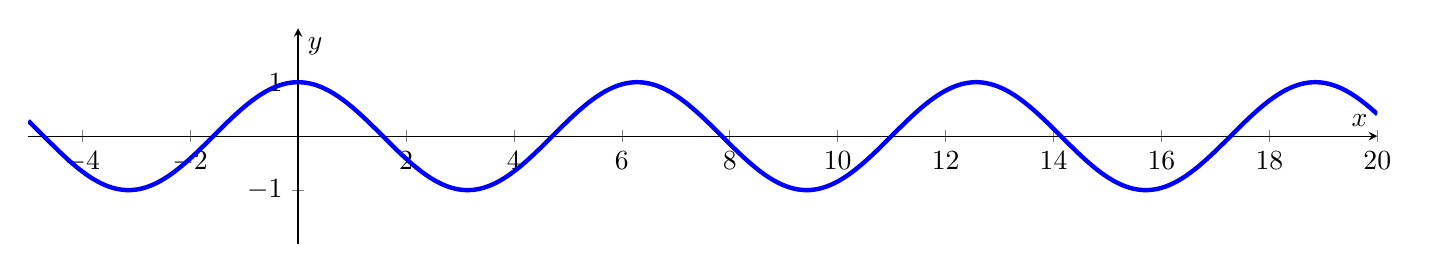
\begin{tikzpicture}
    \begin{axis}[
    scale=2.5,
    axis equal image,
    samples=500,
    axis lines=middle,
    ymin=-2,ymax=2,
    ytick={-1,1},
    ylabel=$y$, 
    xlabel=$x$
    ]
    \addplot[domain=-5:20, black, ultra thick, color=blue] {cos(deg(x))};
    \end{axis}
    \end{tikzpicture}
\end{image}
}

Definities worden met behulp van \verb|\begin{definition}| als volgt weergegeven:

\begin{definition}[Absolute waarde]\label{showcase:absolutewaarde}\nl 

	Voor een reëel getal $a\in\R$ definiëren we de \textit{absolute waarde} van $a$, genoteerd $|a|$, als
	\[
		|a| \perdef\displaystyle\ 
		          \left\{
			\begin{array}{rll  } 
				a  & \mbox{als} & a \geq 0 \\
				-a & \mbox{als} & a<0.
			\end{array}\right.
	\]
\end{definition}

Opmerkingen daarentegen kunnen gewoon in de doorlopende tekst staan, of via \verb|\begin{remark}|:

\begin{remark}[Eigenschappen van de absolute waarde (met $a\in\R$)] \nl
		\begin{enumerate}
			\item Pas op: $|-a|= |a|$, maar \textit{zeer zeker niet} $\xcancel{|-a|=a}$
			
			$|-a|=a$ is \textsc{fout} als $a<0$. Inderdaad,  als $a=-7$, dan is $|-a| = |-(-7)| {\color{red}\neq} -7 = a$
			\item $|a^2 + 1| = a^2 + 1$, want $a^2+1$ is altijd positief.
			% \item $|a^2 - 1| = ....$ \qquad(er is \textsc{geen} eenvoudige algemene formule zonder $|\cdot|$)
\end{enumerate}
\end{remark}

Voorbeelden gebruiken \verb|\begin{example}|. Ze kunnen online meerkeuzeopties bevatten die in de PDF als gewone doorlopende tekst worden weergegeven.
Voor voorbeelden wordt trouwens per default ook in de handout-versie het juiste antwoord al gegeven, terwijl dat voor de oefeningen natuurlijk niet het geval is.
    
\renewcommand{\choiceminimumverticalsize}{\vphantom{$\sqrt{2}$}} 

\begin{example}[Eenvoudige voorbeelden van absolute waarden] \nl 
	
\begin{xmmulticols}
		\begin{enumerate}
			\item $|5|=5$ en $|-5|=5$
			\item $|\sqrt{2}-1| = $\onlineChoice{\choice[correct]{$\sqrt{2} - 1$}\choice{$1-\sqrt{2}$}}
			\item $|1-\sqrt{2}| = $\wordChoice{\choice[correct]{$\sqrt{2} - 1$}\choice{$1-\sqrt{2}$}}
			\item $|2-\sqrt{2}| = $\wordChoice{\choice{$\sqrt{2} - 2$}\choice[correct]{$2-\sqrt{2}$}}
		\end{enumerate}
\end{xmmulticols}
\end{example}

\begin{exercise}[Eenvoudige oefeningen over absolute waarden] \nl 
	
    \begin{xmmulticols}
    \begin{question} $|2-5| = \answer{3}$ \end{question}
    \begin{question} $|5-2| = \answer[onlineshowanswerbutton]{3}$ \end{question}
    \begin{question} $|5-\sqrt{2}| = \answer[onlinenoinput]{3.58578643763}$ \end{question}
    \begin{question} 
        $|1-\sqrt{2}| = $\wordChoice{\choice[correct]{$\sqrt{2} - 1$}\choice{$1-\sqrt{2}$}}
    \end{question}
    \end{xmmulticols}
\end{exercise}
    

In de pdf kan de stijl worden aangepast via alle standaard LaTeX mogelijkheden. Voor de online versie bestaat de mogelijkheid zelf css files toe te voegen:
	\begin{itemize}
		\item \verb|global.css| in de root map van de repository: alle modules in de repository gebruiken deze styling
		\item \verb|xoursefilename.css| in de folder van xoursefilename.tex file: alle modules in de xourse gebruiken deze styling
		\item \verb|activityfilename.css| in de folder van de activityfilename.tex file: styling specifiek voor 1 activity.
	\end{itemize}
%	De \verb|ximeraShowcase.css| file specifieert in dit geval dat de questions niet alleen links maar ook rechts een paarse balk hebben. 
    % niet het geval ...?



\end{document}
